\part{Analyse des résultats}


\section{Etude de la stabilité}

Dans cette partie, nous allons évaluer la stabilité de chaque modèle numérique qui nous permettra d'étudier les conditions de convergence de ces différents modèles expérimentaux à partir des paramètres de discrétisation.


En effet, la stabilité dépend du Courant- Friechichs-Lewy (CFL), condition suffisante de la stabilité liant les pas d'espace $\Delta x $ et de temps $\Delta t$ . Le CFL est une condition de convergence pour résoudre certaines équations aux dérivées partielles.\\

Dans notre problème le CFL est défini de la façon suivante:

\begin{minipage}{.6\textwidth}%
\centering
\begin{equation*}
     \alpha= c \frac{\Delta t}{\Delta x}  
\end{equation*}

\end{minipage}
\hfill
\begin{minipage}{.45\textwidth}%
\vspace{7mm}
$c$: célérité de l'onde $x$\\
$\Delta x$: pas d'espace\\
$\Delta t$ : pas de temps\\
     
\end{minipage}

Les tests ont été effectués avec des valeurs de référence:
\begin{itemize}
    \item c=340 m/s (vitesse d'une onde dans l'air)
    \item L=0.5 m (longueur moyenne d'une corde de guitare)
    \item Durée=0.001 s\\ 
\end{itemize}
Et avec les conditions initiales suivantes:
  \[
      \begin{cases}
        u^{0}_{i}=\sin(\frac{n \pi }{L} \times i \times \Delta x) \\
        \frac{\partial u^0_{i}}{\partial t}= 0
      \end{cases}
    \]\\


\subsection{Méthodes d'Euler}

Pour étudier la stabilité de cette méthode, nous allons faire varier d'abord  $\Delta t$  puis $\Delta x$ pour obtenir les graphiques les plus précis pour chaque schéma explicite et implicite, l'objectif étant de trouver un compromis entre l'efficacité et la précision.

\subsubsection{Schéma explicite}

$\triangleright$\textbf{Variation de  $\Delta t$(en secondes) à $\Delta x$(en mètres) fixé :}\\

\begin{enumerate}[label=\alph*)]
\begin{minipage}{.5\textwidth}%

\item $\Delta x =  5*{10}^{-4}m$\\
$\Delta t$ = ${10}^{-2} s $\\
$\alpha$ =$6,8*{10}^{3}$\\

$\Longrightarrow$ On obtient aucune représentation.

\end{minipage}


\begin{minipage}{.5\textwidth}%

\item $\Delta x = 5*{10}^{-4}m$\\
$\Delta t$ = ${10}^{-5} s $ \\
$\alpha =6,8$\\

$\Longrightarrow$ On obtient une surface plane.\\
Temps d'exécution =$0,11s$


\end{minipage}%
\hfill
\begin{minipage}{.45\textwidth}%
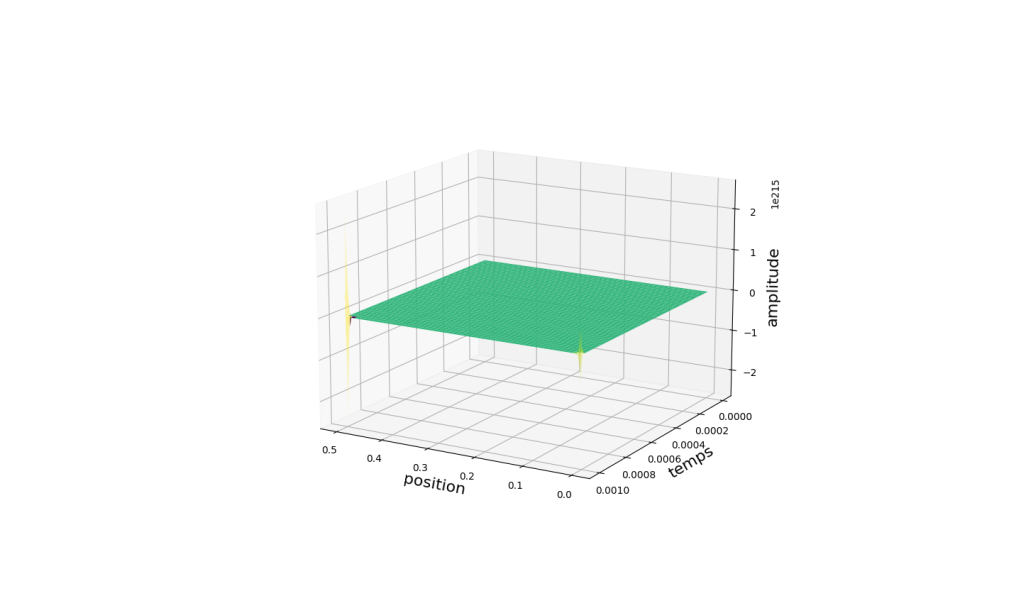
\includegraphics[width=12cm,height=6cm]{explicited.png}

\end{minipage}%

\begin{minipage}{.5\textwidth}%

\item $\Delta x$ = $5*{10}^{-4}m$\\
$\Delta t$=${10}^{-6} s $ \\
$\alpha$=$6,8*{10}^{-1}s$\\

$\Longrightarrow$ On obtient une courbe parfaitement sinusoidale.\\
Temps d'exécution = $1,24s$

\end{minipage}%
\hfill
\begin{minipage}{.45\textwidth}%
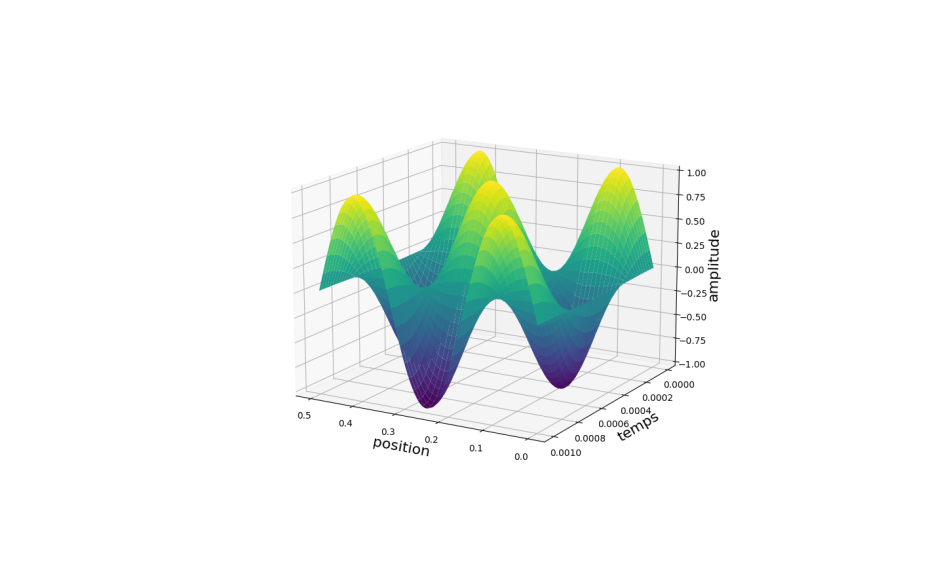
\includegraphics[width=12cm,height=6cm]{explicitee.png}

\end{minipage}%

\begin{minipage}{.5\textwidth}%


\item $\Delta x$=$5*{10}^{-4}m$\\
$\Delta t={10}^{-8}$\\
$\alpha$=$6,8*{10}^{-3}s$\\


$\Longrightarrow$ On obtient une courbe parfaitement sinusoidale.\\
Temps d'exécution =$122s$
\end{minipage}%
\hfill
\begin{minipage}{.45\textwidth}%
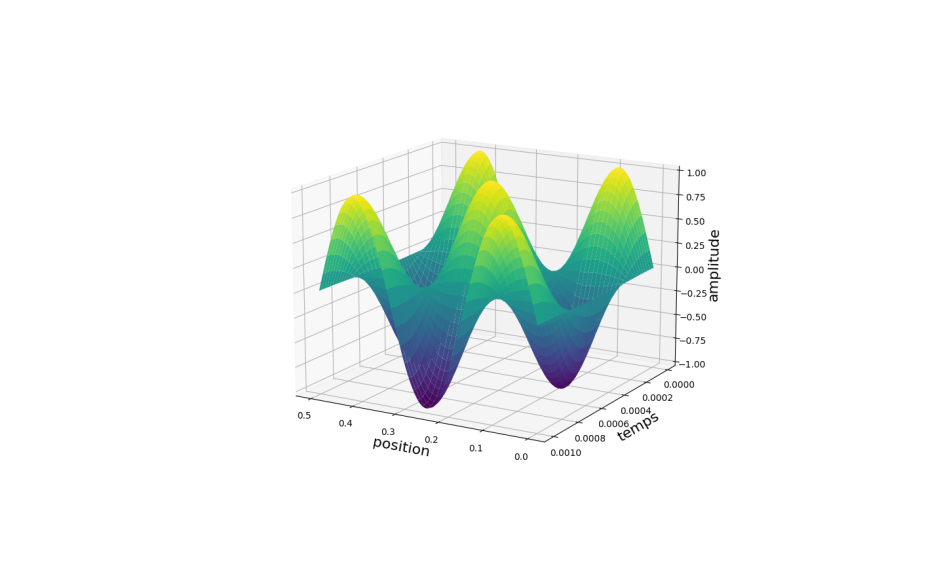
\includegraphics[width=12cm,height=6cm]{explicitee.png}
\end{minipage}%



\end{enumerate}
D'aprés ces différents tests, on peut remarquer que le schéma est de plus en plus sinusoïdale lorsque le CFL se rapproche de 1.\\



$\triangleright$\textbf{Variation de  $\Delta x$ à $\Delta t$ fixé :}\\

On fixe $\Delta t$ à différentes valeurs:\\

\hspace*{1cm}$\bullet$ Pour $\Delta t= {10}^{-3}$ \\

\begin{enumerate}[label=\alph*)]

\begin{minipage}{.6\textwidth}%

\item $\Delta x=3,4*{10}^{-2}m$ \\
$\Delta t= {10}^{-4}$ \\
$\alpha= 1$\\


$\Longrightarrow$ On obtient aucun affichage.

\end{minipage}%
\hfill
\begin{minipage}{.6\textwidth}%

\item $\Delta x=7*{10}^{-2}m$ \\
$\Delta t= {10}^{-4}$ \\
$\alpha= 4,8*{10}^{-1}m$\\


$\Longrightarrow$ On obtient aucun affichage.\\

\end{minipage}%


\end{enumerate}

\vspace*{1cm}
\hspace*{1cm}$\bullet$ Pour $\Delta t= {10}^{-6}$ \\

\begin{enumerate}[label=\alph*)]

\begin{minipage}{.45\textwidth}%

\item $\Delta x=4*{10}^{-3}m$ \\
$\Delta t= {10}^{-6}$ \\
$\alpha= 0,85$\\


$\Longrightarrow$ On obtient la representation d'une onde parfaitement sinusoïdale.\\
Temps d'exécution = $0,043s$

\end{minipage}%
\hfill
\begin{minipage}{.6\textwidth}%
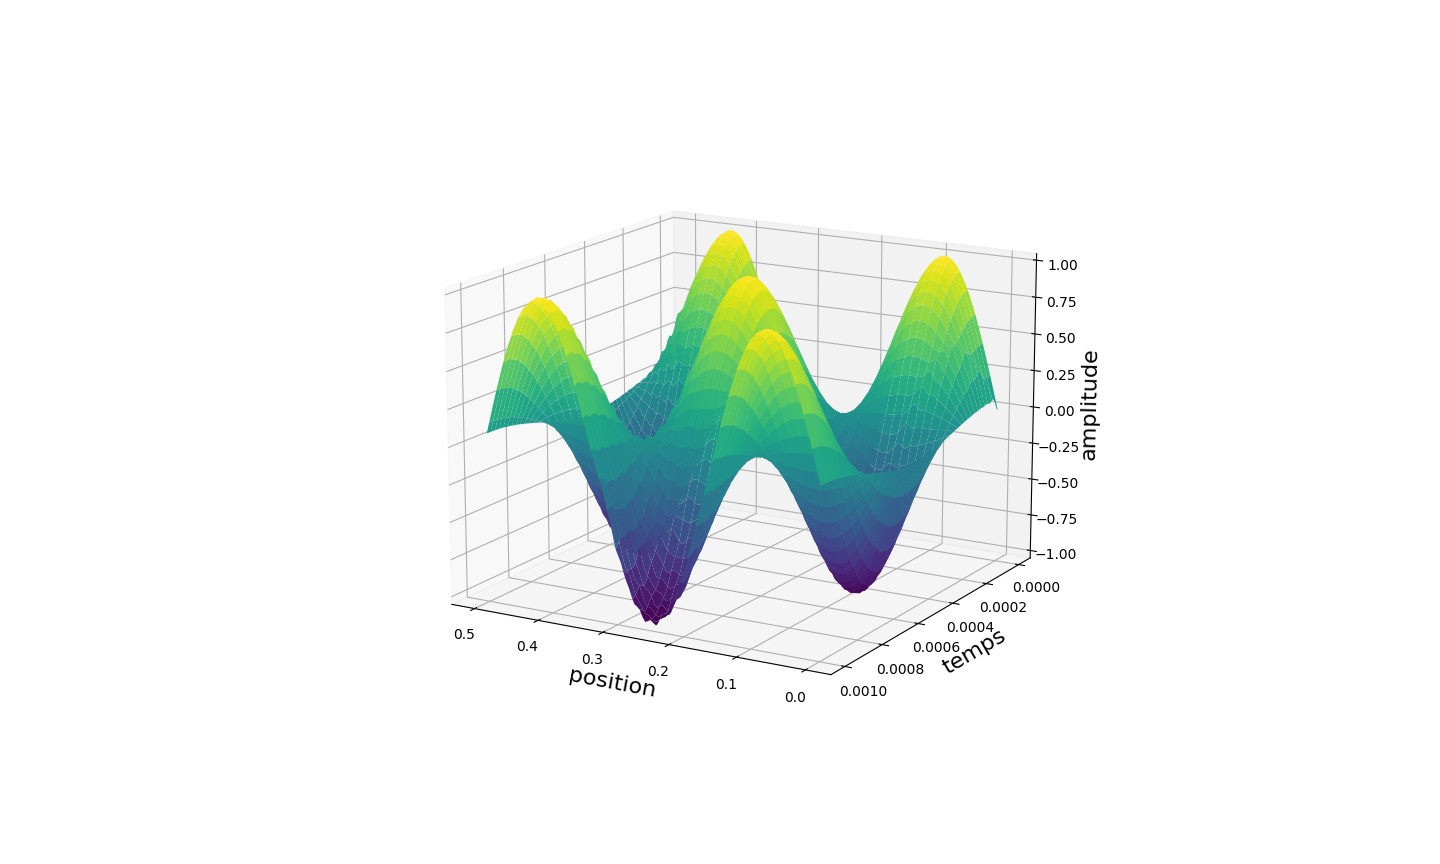
\includegraphics[width=12cm,height=6cm]{dt=10^-6 et dx=0.004.png}

\end{minipage}%
\newline
\begin{minipage}{.45\textwidth}%
\item $\Delta x=4*{10}^{-2}m$ \\
$\Delta t= {10}^{-6}$ \\
$\alpha= 0,0085$\\


$\Longrightarrow$ On obtient une figure sinusoïdale.\\
Temps d'exécution = $0,016s$

\end{minipage}%
\begin{minipage}{.45\textwidth}%
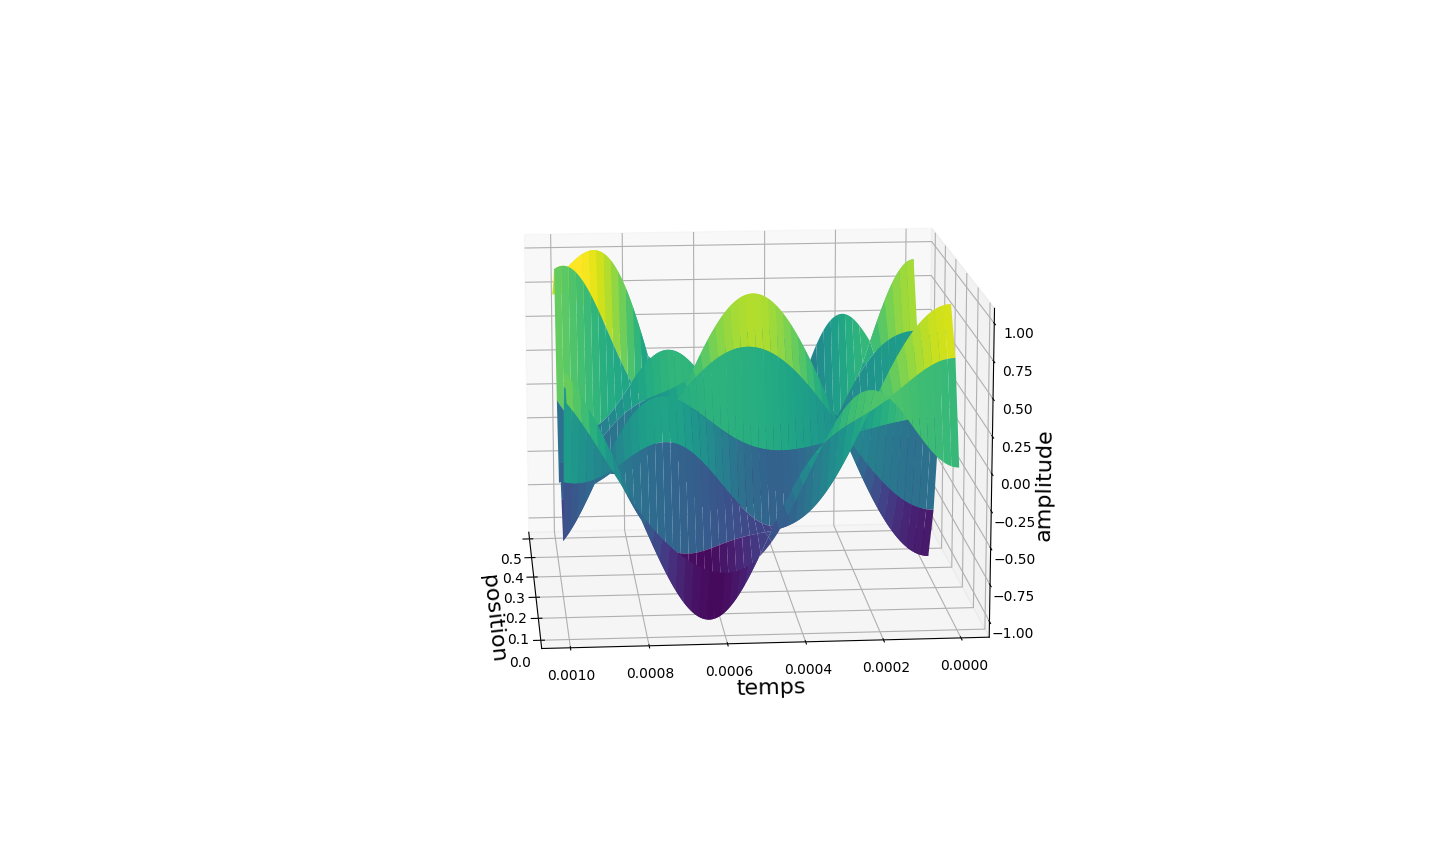
\includegraphics[width=12cm,height=6cm]{dt=10^-6 avec dx=0.04.png}

\end{minipage}%

On constate à travers ces différents tests concernant la variation de l'espace à $\Delta t$ fixé, que les représentations se modélisent de mieux en mieux lorsque notre dt décroit.


\end{enumerate}


\subsubsection{Schéma implicite :}

$\triangleright$ \textbf{Variation de $\Delta t$ (en secondes) à $\Delta x$ (en mètres) fixé :}\\
\begin{enumerate}[label=\alph*)]


\begin{minipage}{.5\textwidth}%

\item $\Delta x =  5*{10}^{-4}m$\\
$\Delta t$ = ${10}^{-2} s $\\
$\alpha$ =$6,8*{10}^{3}$\\

$\Longrightarrow$ Représentation non supportée donc aucun affichage car $\alpha$ est trop grand.\\ 

\end{minipage}%




\begin{minipage}{.5\textwidth}%
\item $\Delta x = 5*{10}^{-4}m $\\
$\Delta t$ = ${10}^{-4}m s $ \\
$\alpha =68$ \\

$\Longrightarrow$ En ayant un $\alpha$ qui se rapproche de 1, on obtient une onde partiellement sinusoïdale.\\
Temps d'exécution = $0,207s$

\end{minipage}%
\hfill
\begin{minipage}{.45\textwidth}%
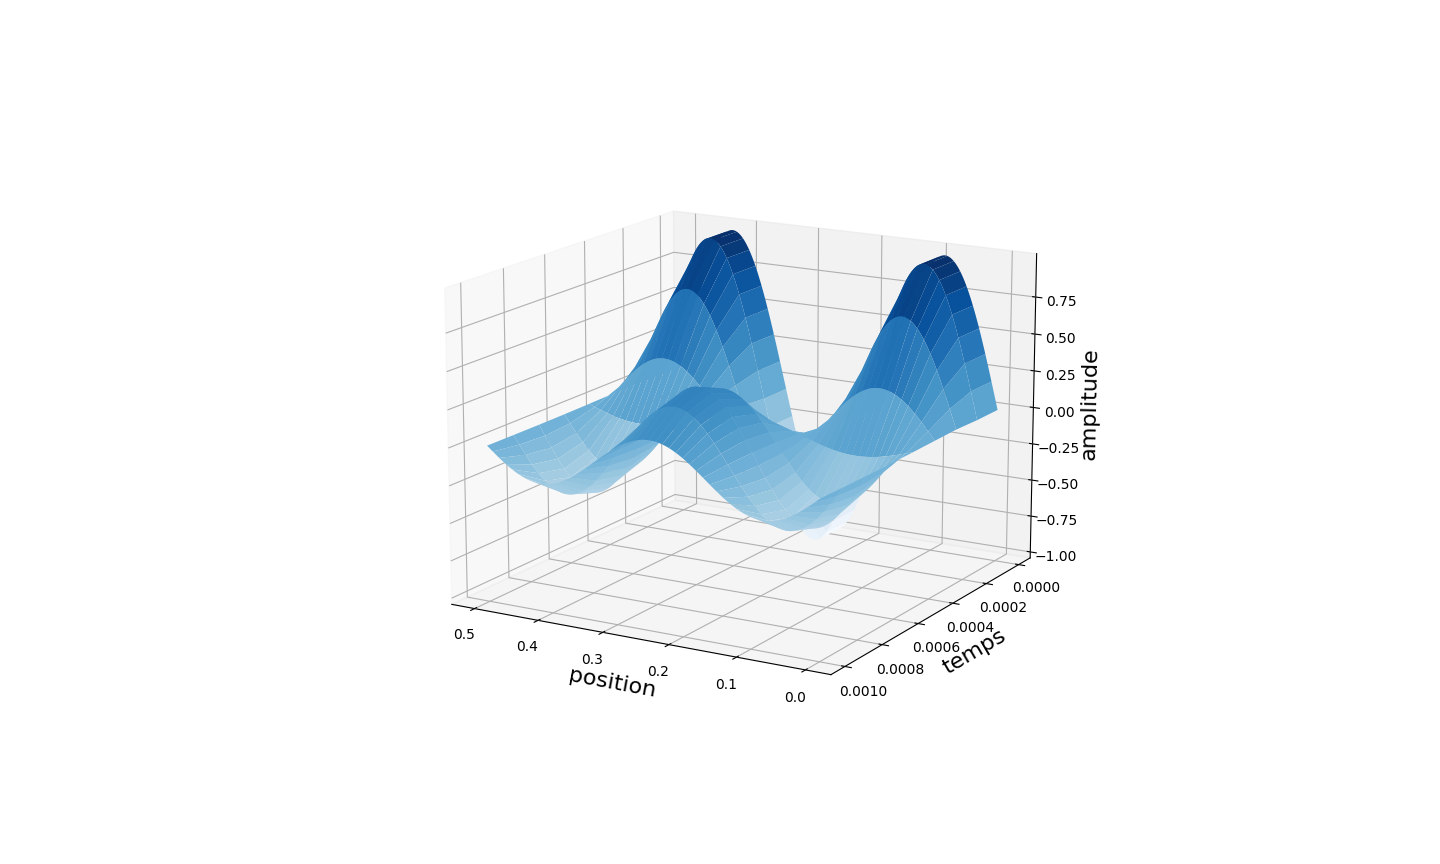
\includegraphics[width=10cm,height=6cm]{implicitec.png}
\end{minipage}%

\begin{minipage}{.5\textwidth}%
\item $\Delta x = 5*{10}^{-4}m$\\
$\Delta t$ = ${10}^{-5} s $ \\
$\alpha =6,8$\\

$\Longrightarrow$ On obtient une surface parfaitement  sinusoïdale lorsque le pas de temps est plus petit et donc par conséquent un $\alpha$ plus petit se rapprochant de 1.\\ 
Temps d'exécution = $0,302s$
\end{minipage}%
\hfill
\begin{minipage}{.45\textwidth}%
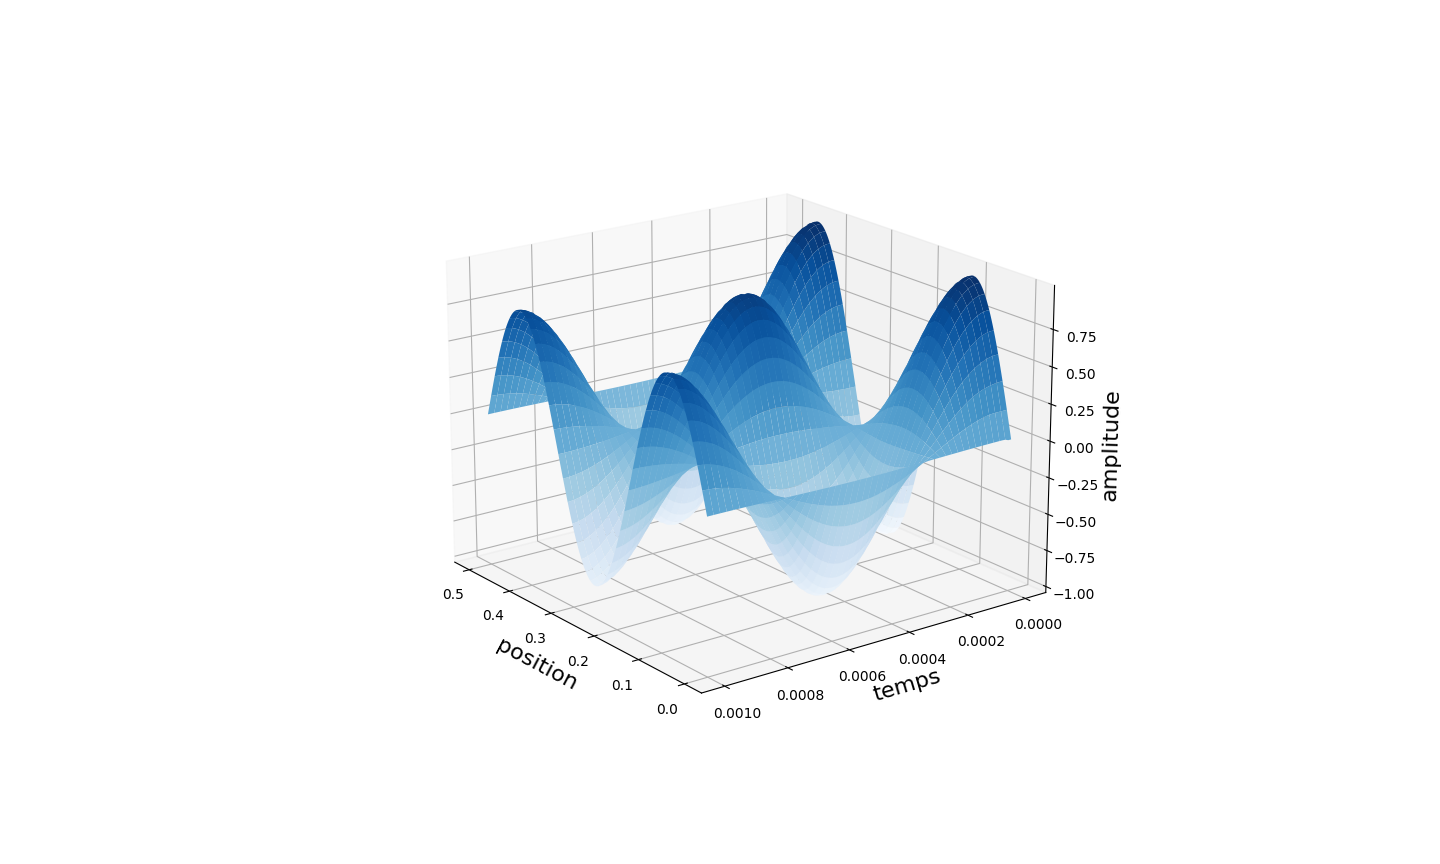
\includegraphics[width=10cm,height=6cm]{implicited.png}
\end{minipage}%




\begin{minipage}{.8\textwidth}%

\item $\Delta x=5*{10}^{-4}m$\\
$\Delta t$=${10}^{-8}$\\
$\alpha$=$6,8*{10}^{-3}s$\\


$\Longrightarrow$On obtient aucune représentation de l'onde car le pas de $\alpha$ est trop petit.\\

\end{minipage}%
\newline
\newline
Le coefficient CFL joue un rôle très important dans la stabilité du modéle, ce dernier liant les pas de temps et d'espace nous permet d'avoir des représentations plus ou moins sinusoïdales en fonction de la variation de $\Delta t$.
\end{enumerate}

$\triangleright$\textbf{Variation de  $\Delta x$ à $\Delta t$ fixé :}\\

\begin{enumerate}[label=\alph*)]

\hspace*{1cm}$\bullet$ Pour $\Delta t= {10}^{-3}$ \\
\newline

\begin{minipage}{.6\textwidth}%

\item $\Delta x=5*{10}^{-3}m$ \\
$\Delta t= {10}^{-3}$ \\
$\alpha= 680$\\


$\Longrightarrow$ On obtient aucun affichage.

\end{minipage}%

\begin{minipage}{.45\textwidth}%

\item $\Delta x=3*{10}^{-2}m$ \\
$\Delta t= {10}^{-5}$ \\
$\alpha= 1,1*{10}^{-1} $\\


$\Longrightarrow$ On commence à avoir une forme d'onde sinusoïdale. 

\end{minipage}%
\hfill
\begin{minipage}{.6\textwidth}%
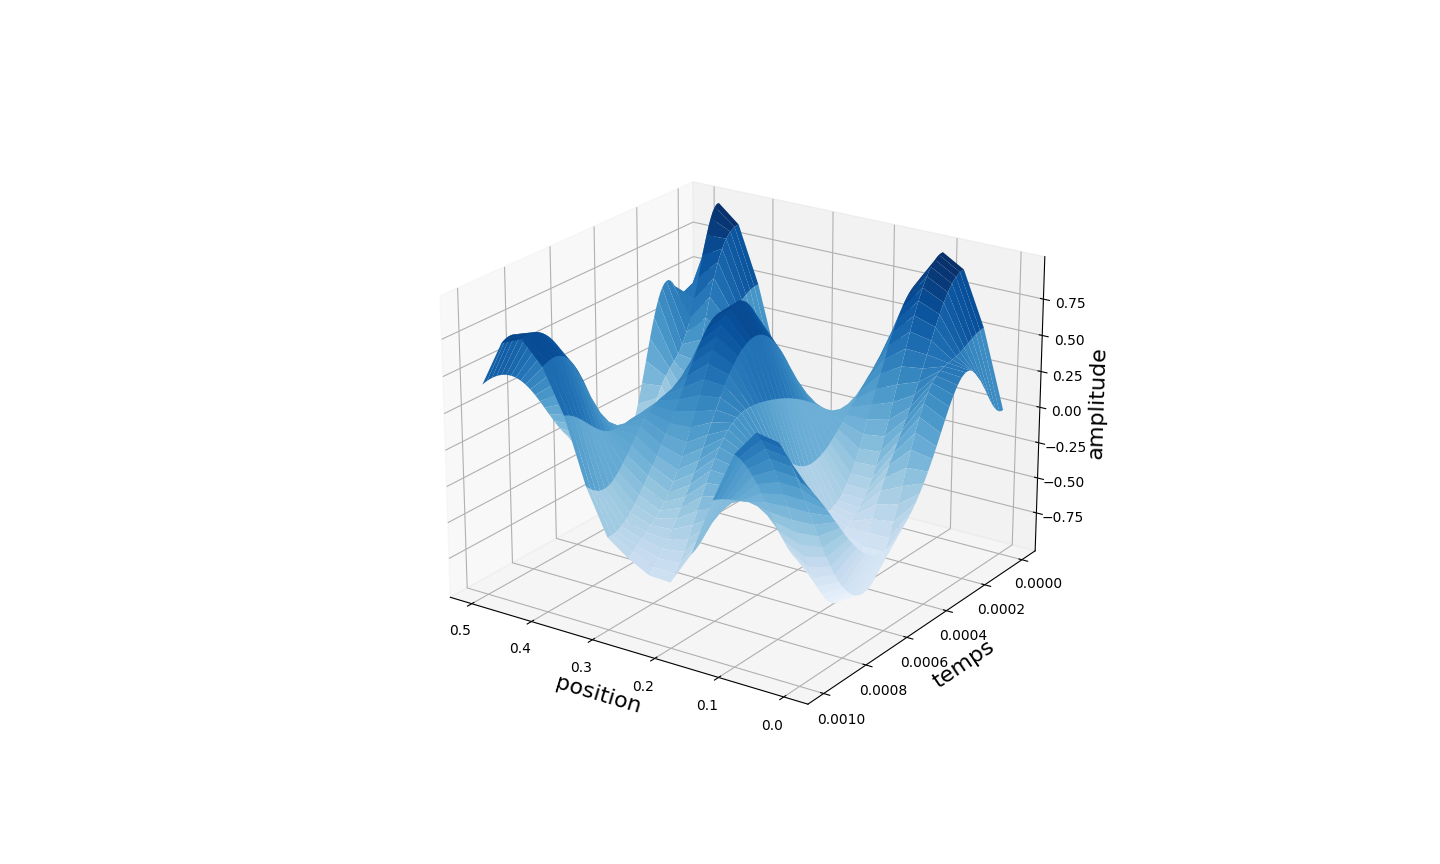
\includegraphics[width=12cm,height=6cm]{dt=0.00001 avec dx=0.03.png}
\end{minipage}%


\hspace*{1cm}$\bullet$ Pour $\Delta t= {10}^{-5}$ \\

\begin{minipage}{.45\textwidth}%
\item $\Delta x=9*{10}^{-2}m$\\
$\Delta t={10}^{-5}$\\
$\alpha= 0,03$ \\
$\Longrightarrow$ L'onde commence à apparaître de maniére imprécise.
\end{minipage}%
\hfill
\begin{minipage}{.6\textwidth}%
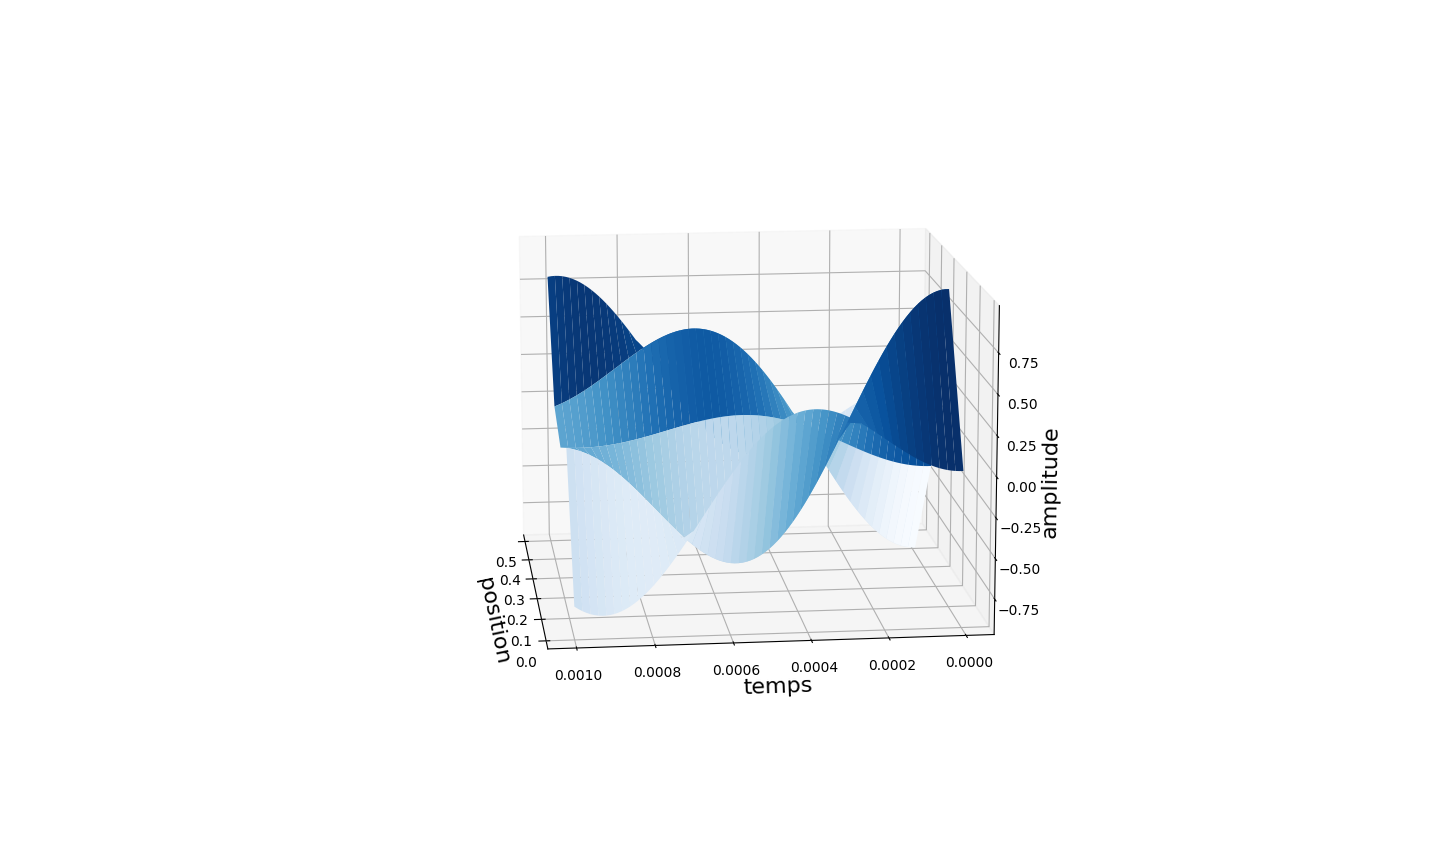
\includegraphics[width=12cm,height=6cm]{dt=0.00001 et dx=0.09.png}
\end{minipage}%

\hspace*{1cm}$\bullet$ Pour $\Delta t= {10}^{-6}$ \\
\begin{minipage}{.45\textwidth}%

\item $\Delta x=7*{10}^{-3}m$ \\
$\Delta t= {10}^{-6}$ \\
$\alpha=0,048s $\\


$\Longrightarrow$ On obtient une représentation parfaitement sinusoïdale.

\end{minipage}%
\hfill
\begin{minipage}{.6\textwidth}%

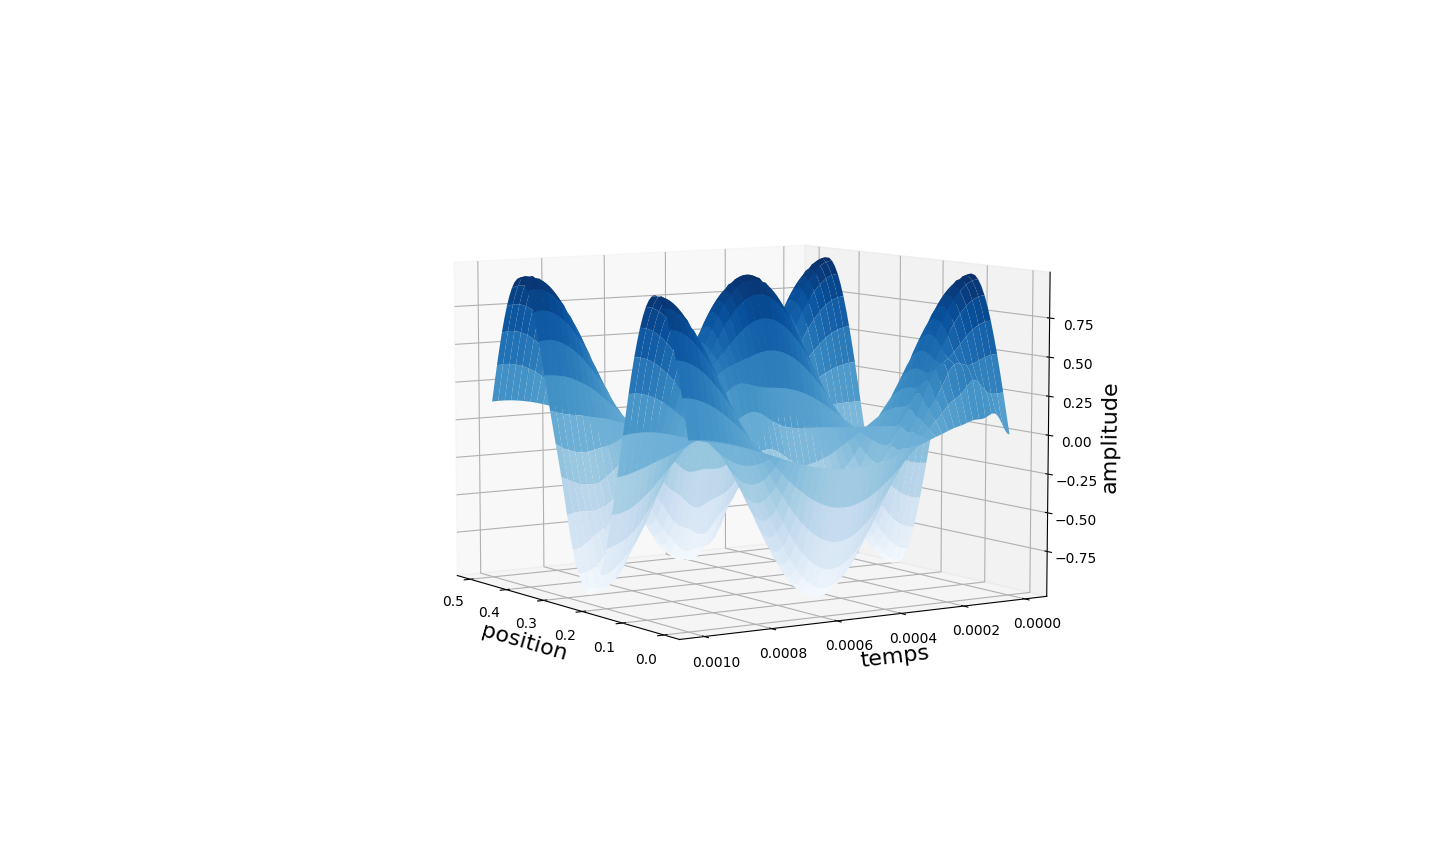
\includegraphics[width=12cm,height=6cm]{dt=10^-6 avec dx= 0.007 .png}
\end{minipage}

\begin{minipage}{.45\textwidth}%

\item $\Delta x=2,4*{10}^{-2}m$ \\
$\Delta t= {10}^{-6}$ \\
$\alpha=1,4*{10}^{-2} $\\


$\Longrightarrow$ On a une représentation sinusoïdale. 
\end{minipage}%
\hfill
\begin{minipage}{.6\textwidth}%

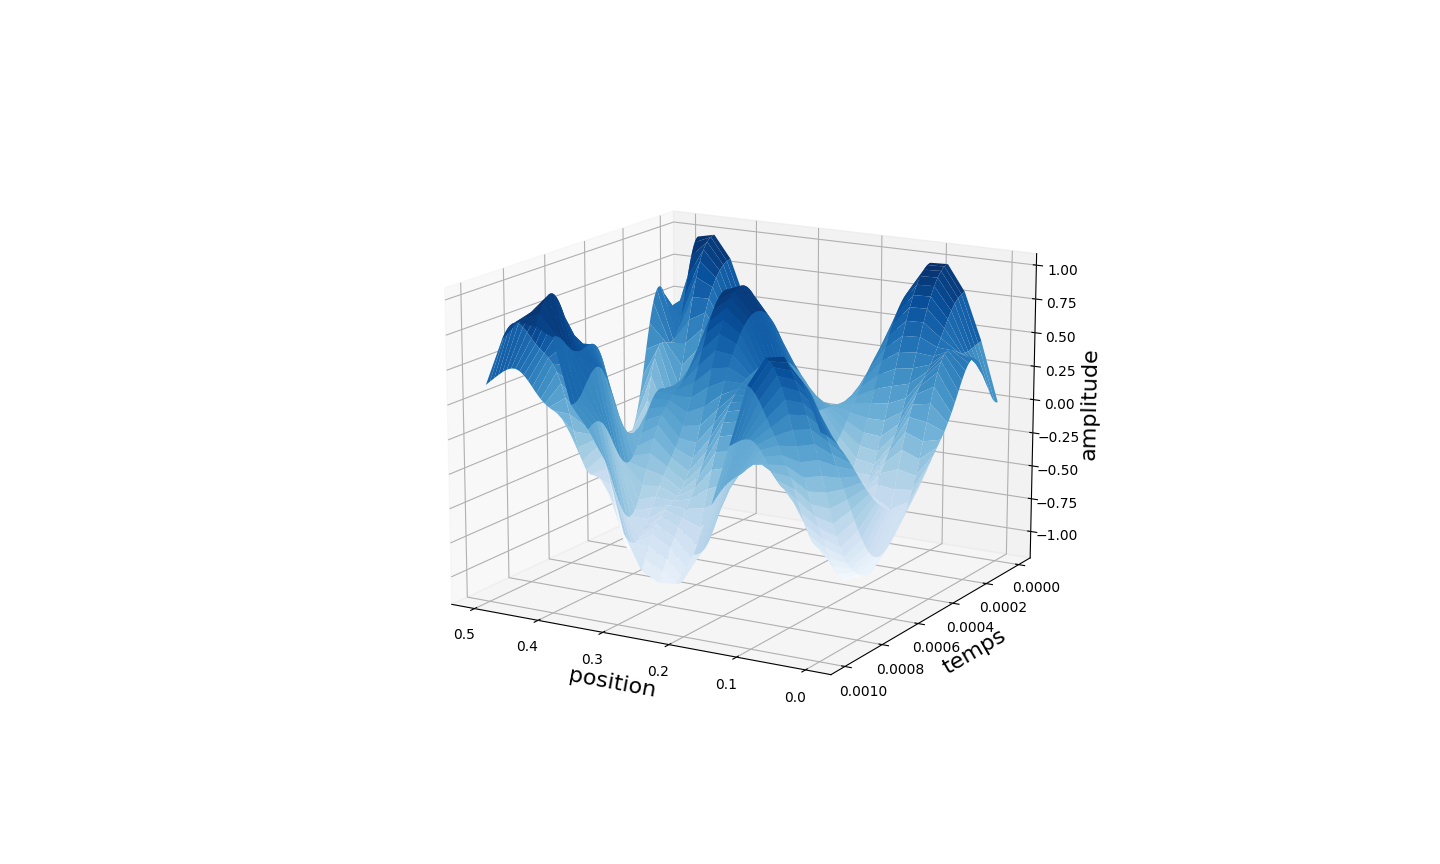
\includegraphics[width=12cm,height=6cm]{dt=10^-6 avec dx=0.024.png}
\end{minipage}
On obtient comme précedemment, une modélisation représentative de la corde lorsque le pas de temps diminue mais également en ayant un pas d'espace d'ordre ${10}^{-2}$\\


\textbf{Conclusion}: On peut remarquer d'aprés cette série de tests, que la stabilité est obtenu généralment avec un coefficient CFL proche de 1 par conséquent un pas d'espace $\Delta x$ de l'ordre ${10}^{-2}$ au minimum et un pas de temps de l'ordre ${10}^{-5}$ au minimum.   


\end{enumerate}

\subsection{Méthode de Runge-Kutta}
Le principe d'étude de la stabilité du modèle reste le même que pour les schémas d'Euler. Il faut donc faire varier les pas $\Delta x$ et $\Delta t$ de manière à avoir les meilleurs graphiques.
Mais, il apparaît assez évident que le modèle risque de diverger avec le terme $(\frac{c}{\Delta x})^2$.\\

    
\begin{figure}[H]
\begin{minipage}[b]{.46\linewidth}
\centering\epsfig{figure=33.png,width=7cm}
\caption{
        $\Delta x= 5^{-3}m $\\
        $\Delta t= 10^{-4}s$\\
        $\alpha = 6.8$
    \label{fig1}
    }
\end{minipage} \hfill
\begin{minipage}[b]{.46\linewidth}
\centering\epsfig{figure=11.png,width=7cm}
\caption{$\Delta x= 5^{-3}m $\\ 
        $\Delta t= 10^{-5}s$\\
        $\alpha = 0.68$
        \label{fig2}}
\end{minipage}
\end{figure}

\begin{figure}[H]
\begin{minipage}[b]{.46\linewidth}
\centering\epsfig{figure=6.png,width=7cm}
\caption{$\Delta x= 5^{-2}m $\\ 
        $\Delta t= 10^{-6}s$\\
        $\alpha = 0.0068$
        \label{fig1}}
\end{minipage} \hfill
\begin{minipage}[b]{.46\linewidth}
\centering\epsfig{figure=8.png,width=\linewidth}
\caption{$\Delta x= 5^{-3} m $\\ 
        $\Delta t= \frac{\Delta x}{c}s= 1.47.10^{-5} $\\
        $\alpha = 1$
        \label{fig2}}
\end{minipage}
\end{figure}


A partir des simulations effectuées (les autres étant en annexe 5), est possible d'observer expérimentalement les conditions de stabilité du modèle construit.
\begin{enumerate}
    \item Par rapport au CFL : $\alpha = c\frac{\Delta t}{\Delta x}$\\
    On peut remarquer que le modèle est "correct" uniquement lorsque $\alpha < 1 $  (Figure 2).\\
    Dans les autres cas, le résultat est loin de ce qui attendu. Cela est logique étant donné qu'il s'agit ici d'une méthode à deux pas, donc le CFL est un paramètre important.
    \item Par rapport aux valeurs  de $\Delta t$ et $\Delta x$ \\
    On peut remarquer que la stabilité du modèle augmente lorsque le pas $\Delta t$ diminue, il faut que $\Delta t$ soit plus petit que $\Delta x$ et que $\Delta x$ soit assez petit mais pas trop par rapport à $\Delta t$.\\
    Cela découlerait de l'utisation de la méthode de Runge-Kutta pour la résolution de l'équation.
    
\end{enumerate}


\section{Comparaison des méthodes}
L'objectif principal du projet est de comparer les différentes méthodes de résolution numérique pour l'équation d'onde appliquée à une corde de guitare.
Pour cela, nous allons dans un premier temps comparer expérimentalement les erreurs obtenues pour chaque modèle pour des conditions de stabilité optimales et pour une solution exacte donnée.
Dans un second temps, nous pouvons également comparer les modèles en terme de performance, en considérant la durée d'exécution.

\subsection{Etude des erreurs}
Pour effectuer les calculs d'erreurs, nous avons choisi la fonction suivante :
\begin{equation*}
    u_{exact}(x,t)=cos(\frac{3 \pi c}{L}t)sin(\frac{3 \pi }{L}x )
\end{equation*}
Et donc l'erreur numérique est simplement donnée par :
     $E=|u_{exact} - u_{num}|$

Ainsi, on obtient comme conditions initiales pour les trois modèles:
  \[
      \begin{cases}
        u^{0}_{i}=\sin(\frac{n \pi }{L} \times i \times \Delta x) \\
        \frac{\partial u^0_{i}}{\partial t}= 0
      \end{cases}
    \]\\
Et les paramètres des modèles sont les suivants:
\begin{itemize}
    \item c=340 m/s (vitesse d'une onde dans l'air)
    \item L=0.5 m (longueur moyenne d'une corde de guitare)
    \item Durée=0.001 s\\ 
\end{itemize}
Et les paramètres de discrétisation pour les méthodes d'Euler sont:
\begin{itemize}
    \item $\Delta x=0.0005$
    \item $\Delta t=\frac{\Delta x}{c}$
\end{itemize}
Ceux de la méthode de Runge-Kutta sont: 
\begin{itemize}
    \item $\Delta x=0.005$
    \item $\Delta t=0.000001$
\end{itemize}

L'on pourra retrouver les graphiques des solutions pour ces 4 méthodes de calcul en annexe 2.


On peut déjà remarquer que pour les 3 modèles, les solutions numériques sont très proches de la solution exacte en terme de forme de surface mais aussi en terme d'amplitude.


Voici les résultats donnés par les calculs d'erreurs numériques en 3 dimensions.
\begin{figure}[H]
\begin{minipage}[b]{.46\linewidth}
\centering\epsfig{figure=1_comp.png,width=7cm}
\caption{Euler explicite
    \label{fig1}
    }
\end{minipage} \hfill
\begin{minipage}[b]{.46\linewidth}
\centering\epsfig{figure=2_comp.png,width=7cm}
\caption{Euler implicte\label{fig2}}
\end{minipage}
\end{figure}


\begin{figure}[H]
\begin{center}
\begin{minipage}[b]{.46\linewidth}
\centering\epsfig{figure=3_comp.png,width=7cm}
\caption{Runge-Kutta\label{fig1}}
\end{minipage} \hfill
\end{center}
\end{figure}

Les erreurs pour chaque modèle prennent des formes différentes.
Pour les méthodes d'Euler, on peut observer des structures "sinusoïdales" quasiment périodiques. On peut cependant observer sur le schéma explicite une diminution générale de l'erreur à partir d'une certaine position.
Pour le schéma de Runge-Kutta, on retrouve une forme similaire à celle de la méthode d'Euler explicite avec également la même diminution de l'erreur.
\newline
Mais il est plus intéressant d'évaluer les erreurs en 2 dimensions selon le temps. Ainsi, nous avons étudié les moyennes des erreurs pour chaque temps donné.
\newline
Les moyennes des erreurs pour chaque t donnés nous donnent alors les graphiques suivants:

\begin{figure}[H]
\begin{center}
\centering\epsfig{figure=7.comp.png,width=15cm}
\caption{Les erreurs pour les 3 méthodes\label{fig1}}
\end{center}
\end{figure}

Les erreurs en fonction de t nous permettent de voir que le modèle le plus précis est le modèle d'Euler explicite.
\newline
Globalement les erreurs ont bien des profils sinusoïdaux mais elles augmentent en fonction du temps, ce qui montre que les modèles présentent des facteurs de propagation d'erreur.
Le modèle le moins précis est le modèle de Runge-Kutta.
\newline
L'ordre des erreurs est de $10^-2$ pour les modèles mais le modèle de Runge-Kutta a une erreur qui croît beaucoup plus vite.

\vspace{1cm}
\subsection{Ordre des erreurs}
Pour finir la comparaison des modèles, nous pouvons déterminer et comparer l'ordre de leurs erreurs.
Pour cela, nous pouvons étudier les expressions suivantes:
\begin{enumerate}
    \item $max|e^n_{i}|$ pour 0<i<Nx et 0<n<Nt en faisant varier le nombre de point de temps Nt
    \item $max|e^n_{i}|$ pour 0<i<Nx et 0<n<Nt en faisant varier le nombre de point de temps Nx
\end{enumerate}

Voici les résultats obtenus:

\begin{figure}[H]
\begin{center}
\centering\epsfig{figure=erreur_dt.png,width=15cm}
\caption{Les erreurs pour des variation de Nt\label{fig1}}
\end{center}
\end{figure}

\begin{figure}[H]
\begin{center}
\centering\epsfig{figure=erreurs_dx.png,width=15cm}
\caption{Les erreurs pour des variation de Nx\label{fig1}}
\end{center}
\end{figure}

A partir de ces résultats, on peut déduire les ordres des erreurs:
\begin{itemize}
    \item Les méthodes d'Euler ont des erreurs selon x et t d'ordre O(N)
    \item La méthode de Runge-Kutta a des erreurs  d'ordre $O(N^2)$ selon t et d'ordre O(N) selon x. On peut remarquer que selon x, l'erreur augmente brutalement au bout d'une certaine valeur, cela est dû au fait que la condition de stabilité du modèle n'est plus respectée.
    \item Globalement la méthode d'Euler explicite est celle qui donne la meilleure précision.
\end{itemize}

Au final, on peut déduire que, dans notre cas, la méthode d'Euler explicite est la plus intéréssante puisqu'elle produit l'erreur la plus petite mais est également efficace en terme d'algorithme contrairement à la méthode de Runge-Kutta qui demande beaucoup plus de calculs pour avoir un résultat cohérent.



\section{Conditions initiales}

\subsection{Variation des conditions initiales}


L'analyse des méthodes utilisés pour la modélisation d'une onde  de corde de guitare repose aussi sur le choix des conditions initiales comme vu précédement.
Un bon choix des conditions initiales est donc indispensable pour avoir une modélisation la plus proche de la réalité ou tout simplement celle qu'on souhaite.\\


Dans cette partie, l'objectif est de tester les différents schémas pour différents profils initiaux de l'onde, qu'on obtiendra en modifiant les conditions initiales. \\

Ainsi, on pourra vérifier les réactions des différents modèles par rapport aux variations de conditions initiales et constater que, tant que les conditons initiales respectent les conditions imposées par le problème $(u(t,x=0)=u(t,x=L)=0)$, on obtient une solution numérique cohérente.\\

Dans un premier temps, on peut considérer une corde pincée en point de l'espace, qui est bien attachée sur les bords.
On peut établir 2 modèles mathématiques différents pour la corde pincée du schéma suivant:

\begin{figure}[H]
\centering
\includegraphics[scale=1]{image2.png}
\caption{Schéma d'une corde pincée}
\label{fig1}
\end{figure}



\begin{enumerate}
    \item Modèle triangulaire
    \begin{equation}
       u(x,t=0)=\left\{
            \begin{array}{ll}
               \ A \frac{x}{x_{0}} &  x\leq x_{0} \\
               \ A \frac{x}{x_{0}} &  x\leq x_{0}
            \end{array}
        \right.
    \end{equation}
    
    
    \item Modèle complet (harpe)
    \begin{equation}
        u(x,t=0)=A\frac{x}{x_{0}}\frac{L-x}{L}
    \end{equation}
    
Dans un deuxième temps, nous allons étudier un troisième modèle où la corde n'est pas accrochée aux bords, c'est-à-dire que, $u(t=0,x=0)$ on a une amplitude $A$ différente de $0$. Le résultat ne devrait alors pas être correct étant donné qu'il ne respecte plus les conditions du problème.
\newline

 \item Modèle "pas accroché aux bords"
    \begin{equation}
       \left\{
            \begin{array}{ll}
               \  u(x,t=0)=cos(\frac{n \pi x}{L})  \\
               \ \frac{\partial{u}}{\partial{t}}(x,t=0)=0 
            \end{array}
        \right.
    \end{equation}
    
    
    
    
    
    
\end{enumerate}


\vspace*{2cm}
\subsection{Implémentation des variations des conditions initiales dans les modéles}


\subsubsection{Méthodes d'Euler}

\subtitle\underline{Euler explicite}



\begin{figure}[H]
\minipage{0.32\textwidth}
  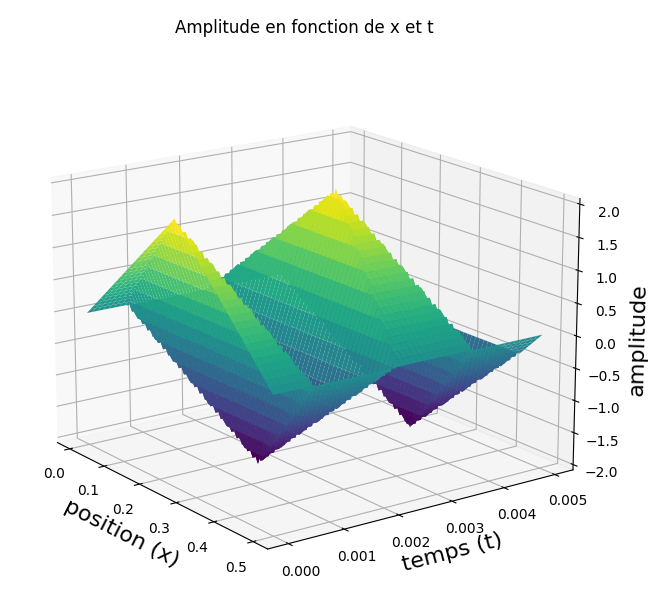
\includegraphics[width=5cm]{1.png}
  \caption{Modèle (1)}\label{fig}
\endminipage\hfill
\minipage{0.32\textwidth}
  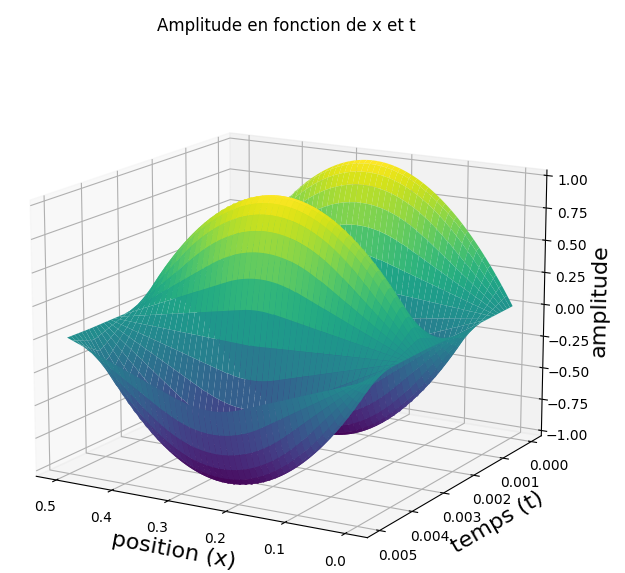
\includegraphics[width=5cm]{2.png}
  \caption{Modèle (2)}\label{fig}
\endminipage\hfill
\minipage{0.32\textwidth}%
  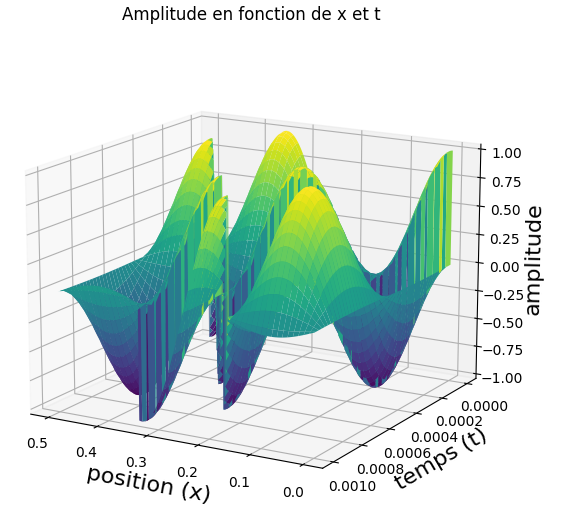
\includegraphics[width=5cm]{7_explicite.png}
  \caption{Modèle (3)}\label{fig}
\endminipage
\end{figure}



\subtitle\underline{Euler implicite}

\begin{figure}[H]
\minipage{0.32\textwidth}
  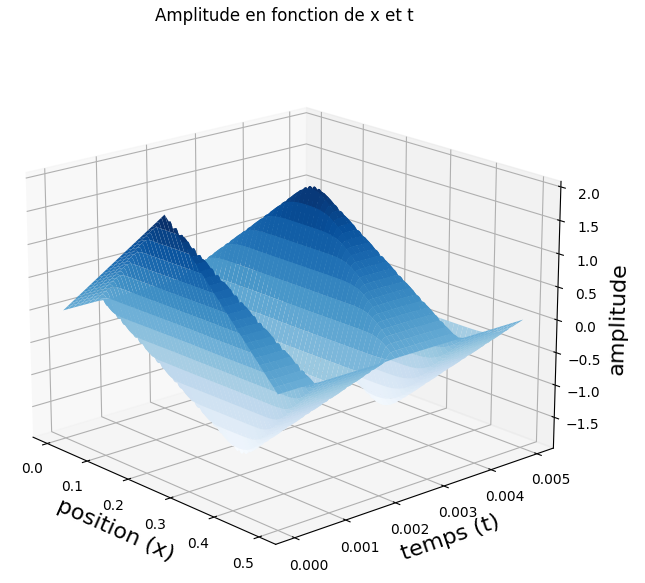
\includegraphics[width=5cm]{3.png}
  \caption{Modèle (1)}\label{fig}
\endminipage\hfill
\minipage{0.32\textwidth}
  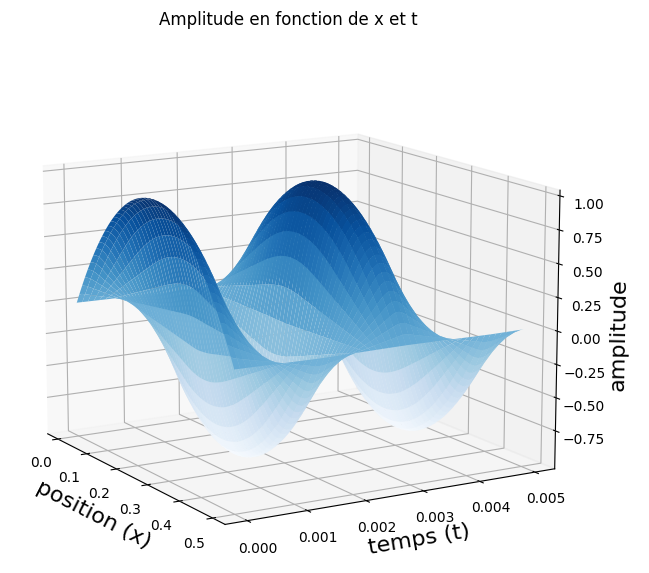
\includegraphics[width=5cm]{4.png}
  \caption{Modèle (2)}\label{fig}
\endminipage\hfill
\minipage{0.32\textwidth}%
  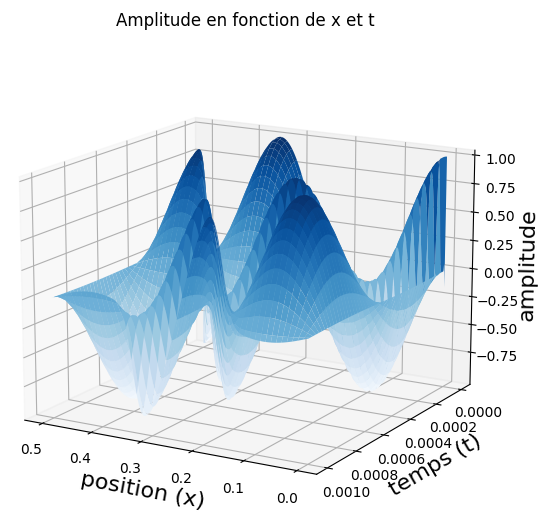
\includegraphics[width=5cm]{8_implicite.png}
  \caption{Modèle (3)}\label{fig}
\endminipage
\end{figure}


\subsubsection{Runge-Kutta}
   
\begin{figure}[H]
\minipage{0.32\textwidth}
  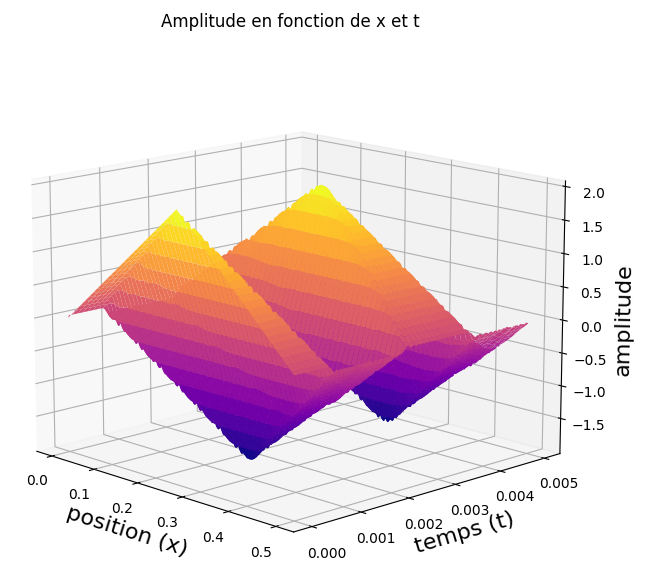
\includegraphics[width=5cm]{5.png}
  \caption{Modèle (1)}\label{fig}
\endminipage\hfill
\minipage{0.32\textwidth}
  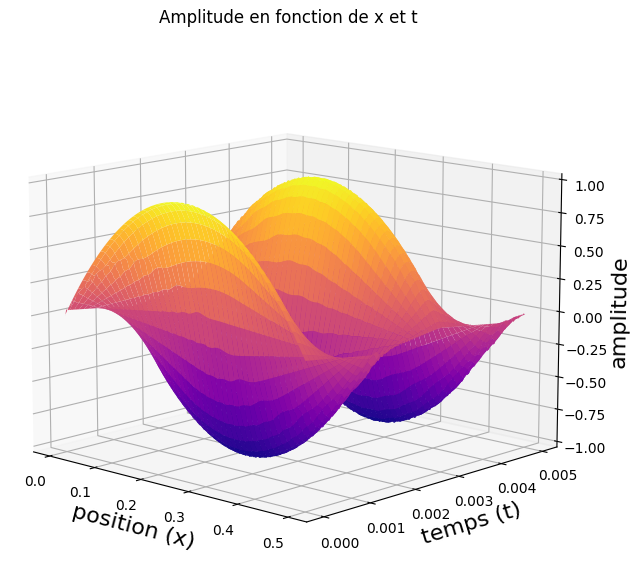
\includegraphics[width=5cm]{6_pro.png}
  \caption{Modèle (2)}\label{fig}
\endminipage\hfill
\minipage{0.32\textwidth}%
  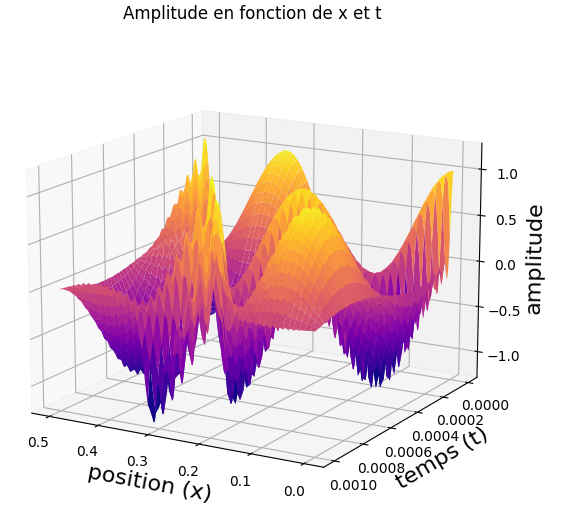
\includegraphics[width=5cm]{9_RK.png}
  \caption{Modèle (3)}\label{fig}
\endminipage
\end{figure}
